\documentclass[epsf,nofootinbib,notitlepage,superscriptaddress]{revtex4-2}
\usepackage{color}
\usepackage{amsmath}
\usepackage{tikz}
\usetikzlibrary{matrix,positioning}
\usepackage{amssymb}

\begin{document}

 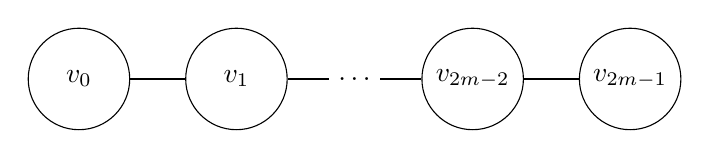
\begin{tikzpicture}[scale=2]

 \begin{scope}[every node/.style={minimum width={width("$v_{2m-1}$")+10pt}}]
    \node[circle, draw] (A) at (0,0) {$v_0$};
    \node[circle, draw] (B) at (1,0) {$v_1$};
	\node[minimum width={10}] (C) at (1.75,0) {$\ldots$}; 
	\node[circle, draw] (D) at (2.5,0) {$v_{2m-2}$};
	\node[circle, draw] (E) at (3.5,0) {$v_{2m-1}$};


\end{scope}

\begin{scope}[every node/.style={scale=1.1}]


\end{scope}
\draw    (A) -- (B);
\draw    (B) -- (C);
\draw    (C) -- (D);
\draw    (D) -- (E);


\end{tikzpicture}

\end{document}